%%%%%%%%%%%%%%%%%%%%%%%%%%%%%%%%%%%%%%%%%
% Beamer Presentation
% LaTeX Template
% Version 1.0 (10/11/12)
%
% This template has been downloaded from:
% http://www.LaTeXTemplates.com
%
% License:
% CC BY-NC-SA 3.0 (http://creativecommons.org/licenses/by-nc-sa/3.0/)
%
%%%%%%%%%%%%%%%%%%%%%%%%%%%%%%%%%%%%%%%%%

%----------------------------------------------------------------------------------------
%	PACKAGES AND THEMES
%----------------------------------------------------------------------------------------

\documentclass{beamer}

\mode<presentation> {

% The Beamer class comes with a number of default slide themes
% which change the colors and layouts of slides. Below this is a list
% of all the themes, uncomment each in turn to see what they look like.

%\usetheme{default}
%\usetheme{AnnArbor}
%\usetheme{Antibes}
%\usetheme{Bergen}
%\usetheme{Berkeley}
%\usetheme{Berlin}
%\usetheme{Boadilla}
%\usetheme{CambridgeUS}
%\usetheme{Copenhagen}
%\usetheme{Darmstadt}
%\usetheme{Dresden}
%\usetheme{Frankfurt}
%\usetheme{Goettingen}
%\usetheme{Hannover}
%\usetheme{Ilmenau}
%\usetheme{JuanLesPins}
%\usetheme{Luebeck}
\usetheme{Madrid}
%\usetheme{Malmoe}
%\usetheme{Marburg}
%\usetheme{Montpellier}
%\usetheme{PaloAlto}
%\usetheme{Pittsburgh}
%\usetheme{Rochester}
%\usetheme{Singapore}
%\usetheme{Szeged}
%\usetheme{Warsaw}

% As well as themes, the Beamer class has a number of color themes
% for any slide theme. Uncomment each of these in turn to see how it
% changes the colors of your current slide theme.

%\usecolortheme{albatross}
%\usecolortheme{beaver}
%\usecolortheme{beetle}
%\usecolortheme{crane}
%\usecolortheme{dolphin}
%\usecolortheme{dove}
%\usecolortheme{fly}
%\usecolortheme{lily}
%\usecolortheme{orchid}
%\usecolortheme{rose}
%\usecolortheme{seagull}
%\usecolortheme{seahorse}
%\usecolortheme{whale}
%\usecolortheme{wolverine}

%\setbeamertemplate{footline} % To remove the footer line in all slides uncomment this line
%\setbeamertemplate{footline}[page number] % To replace the footer line in all slides with a simple slide count uncomment this line

%\setbeamertemplate{navigation symbols}{} % To remove the navigation symbols from the bottom of all slides uncomment this line
}

\AtBeginSection[]{
  \begin{frame}
  \vfill
  \centering
  \begin{beamercolorbox}[sep=8pt,center,shadow=true,rounded=true]{title}
    \usebeamerfont{title}\insertsectionhead\par%
  \end{beamercolorbox}
  \vfill
  \end{frame}
}

\setbeamertemplate{headline}
{
  \leavevmode%
  \hbox{%
  \begin{beamercolorbox}[wd=.5\paperwidth,ht=2.25ex,dp=1ex,right]{section in head/foot}%
    \usebeamerfont{section in head/foot}\thesection\ \insertsectionhead\hspace*{2ex}
  \end{beamercolorbox}%
  \begin{beamercolorbox}[wd=.5\paperwidth,ht=2.25ex,dp=1ex,left]{subsection in head/foot}%
    \usebeamerfont{subsection in head/foot}\hspace*{2ex}\insertsubsectionhead
  \end{beamercolorbox}}%
  \vskip0pt%
}

\usepackage[brazilian]{babel}
\usepackage[utf8]{inputenc}
\usepackage{graphicx} % Allows including images
\usepackage{caption}
\usepackage{subcaption}
\usepackage{booktabs} % Allows the use of \toprule, \midrule and \bottomrule in tables
\usepackage[utf8]{inputenc}
\usepackage{xcolor}
\usepackage{tabularx}
\usepackage{amsmath}
\usepackage{pgfgantt}
\usepackage{hyperref}
\hypersetup{
	   colorlinks=true,    
       urlcolor=cyan,
}
\usepackage{tikz}
\usetikzlibrary{shapes,arrows}
\tikzstyle{decision} = [diamond, draw, fill=blue!20, 
    text width=4.5em, text badly centered, node distance=3cm, inner sep=0pt]
\tikzstyle{block} = [rectangle, draw, fill=blue!20, 
    text width=5em, text centered, rounded corners, minimum height=4em]
\tikzstyle{line} = [draw, -latex']
\tikzstyle{cloud} = [draw, ellipse,fill=red!20, node distance=3cm,
    minimum height=2em]

\newcommand{\norm}[1]{\left\lVert#1\right\rVert}
%----------------------------------------------------------------------------------------
%	TITLE PAGE
%----------------------------------------------------------------------------------------

\title[Trabalho de Graduação 2]{Compressão de Imagens com perda usando Redes Neurais} % The short title appears at the bottom of every slide, the full title is only on the title page

\author[Raphael Soares Ramos]{Raphael Soares Ramos} % Your name
\institute[UnB] % Your institution as it will appear on the bottom of every slide, may be shorthand to save space
{
Universidade de Brasília \\ % Your institution for the title page
\medskip
\textit{raphael.soares@nubank.com.br} % Your email address
}
\date{\today} % Date, can be changed to a custom date

\begin{document}

\begin{frame}
\titlepage % Print the title page as the first slide
\end{frame}

\begin{frame}[allowframebreaks]
\frametitle{Overview} % Table of contents slide, comment this block out to remove it
\tableofcontents % Throughout your presentation, if you choose to use \section{} and \subsection{} commands, these will automatically be printed on this slide as an overview of your presentation
\end{frame}

%----------------------------------------------------------------------------------------
%	PRESENTATION SLIDES
%----------------------------------------------------------------------------------------

%------------------------------------------------
\section{Introdução}
%------------------------------------------------
\subsection{Definições}
%------------------------------------------------
\begin{frame}
\frametitle{Codificação de Dados}
\begin{itemize}
\item Transformação feita nos dados para atingir um certo objetivo.
\item Compressão (redução do comprimento da mensagem) vs. Criptografia (proteger sigilo ou integridade do que os dados significam).
\end{itemize}
\end{frame}
%------------------------------------------------
\begin{frame}
\frametitle{Compressão de Dados}
\begin{itemize}
\item Processo de codificar uma determinada informação utilizando uma menor representação.
\item Arte ou ciência de representar informação de forma compacta~\cite{book_compression}.
\item Duas fases~\cite{book_compression}: modelagem (descrever redundâncias em forma de um modelo) e codificação (codificar descrição do modelo e de como os dados diferem do modelo).
\item Dois tipos: com perda ($x \neq \hat{x}$) e sem perda ($x = \hat{x}$).
\end{itemize}
\end{frame}
%------------------------------------------------
\subsection{Motivação}
%------------------------------------------------
\begin{frame}
\frametitle{Porquê comprimir}
\begin{itemize}
    \item Geração e uso cada vez maior de dados digitais (muitos são redundantes e irrelevantes para determinadas aplicações).
    \item Representar digitalmente 1 segundo de vídeo sem compressão usando o formato CCIR 601 requer mais de 20 \textit{megabytes} de armazenamento ou 160 megabits para transmissão~\cite{book_compression}.
    \item Imagem Monocromática com resolução $512\times512$: $Taxa = \dfrac{512\cdot512\cdot8}{10^6} = 2.097 Mbits$.
    \item Aumentar capacidade de armazenamento e de transmissão de um sistema.
\end{itemize}
\end{frame}
%------------------------------------------------
\subsection{Compressão de Imagens}
%------------------------------------------------
\begin{frame}
\frametitle{Medidas de Desempenho em Compressão de Imagens}
\begin{itemize}
    \item Taxa vs Distorção: $J = D(B) + \lambda R(B)$
    \item Representar com o menor número possívels de bits, preservando a qualidade e a inteligibilidade necessárias à sua aplicação.
    \item \textit{Mean Squared Error} é uma medida comumente usada para distorção.
    \begin{equation} MSE = \dfrac{1}{n}\sum_{n=1}^{N}{(x(n) - \hat{x}(n))}^2 \end{equation}
\end{itemize}
\end{frame}
%--------------------------------------------------
\begin{frame}
\frametitle{Algoritmos de Compressão de Imagens}
\begin{itemize}
    \item Exploram características imperfeitas da nossa percepção e propriedades estatísticas para fornecer resultados superiores quando comparados com métodos de compressão de dados genéricos.
    \item Examinada durante anos por pesquisadores e times como o \textit{Joint Pictures Experts Group}.
    \item Alguns métodos de compressão:
    \begin{enumerate}
    \item JPEG~\cite{jpeg}
    \item JPEG2000~\cite{jpeg2000}
    \item BPG~\cite{bpg}
    \item WebP~\cite{webp}
    \end{enumerate}
\end{itemize}
\end{frame}
%------------------------------------------------
% \subsection{Hipóteses}
% %------------------------------------------------
% \begin{frame}
% \frametitle{Hipóteses}
% \begin{itemize}
%     \item Se modelos baseados em \textit{autoencoders} convolucionais recorrentes são competitivos com os clássicos codecs \textit{JPEG} e \textit{JPEG2000} para imagens com muito conteúdo de alta frequência em determinadas taxas;
%     \item Se o codificador de entropia utilizado no latente será capaz de comprimir em proporções semelhantes para todos as redes de todos os níveis;
%     \item Se ao usar imagens, no treinamento, que codificadores clássicos têm dificuldade para comprimir (imagens com muito conteúdo de alta frequência) é benéfico para os resultados do modelo;
%     \item Se há um grande impacto nos resultados ao usar funções de custo variadas;
% \end{itemize}
% \end{frame}
%--------------------------------------------------
% \subsection{Objetivos}
% %------------------------------------------------
% \begin{frame}
% \frametitle{Objetivo geral}
% \begin{itemize}
% \item Avaliar o desempenho de um \textit{framework} de compressão de imagens ponta a ponta (modelagem e codificação) usando \textit{autoencoders} empilhados convolucionais recorrentes com o auxílio de um codificador de entropia para comprimir o latente binarizado gerado pelo \textit{encoder}.
% \item Comparar com os codecs clássicos \textit{JPEG} e \textit{JPEG2000}.
% \end{itemize}
% \end{frame}
%------------------------------------------------------
\section{Fundamentação Teórica}
%------------------------------------------------------
\subsection{JPEG}
%------------------------------------------------------
% \begin{frame}
% \frametitle{Formato de Arquivos}
% \begin{itemize}
% \item Arquivos comprimidos pelo método \textit{JPEG} são normalmente descritos no formato \textit{JPEG File Interchange Format (JFIF)}, que é uma limitação (um subconjunto) do padrão \textit{JPEG} completo (muitos espaços de cores e modos de operação).
% \begin{enumerate}
% \item Primeiro é feita conversão do espaço de cor para YCbCr.
% \end{enumerate}
% \end{itemize} 
% \end{frame}
%------------------------------------------------------
\begin{frame}
\frametitle{Funcionamento}
\begin{figure}
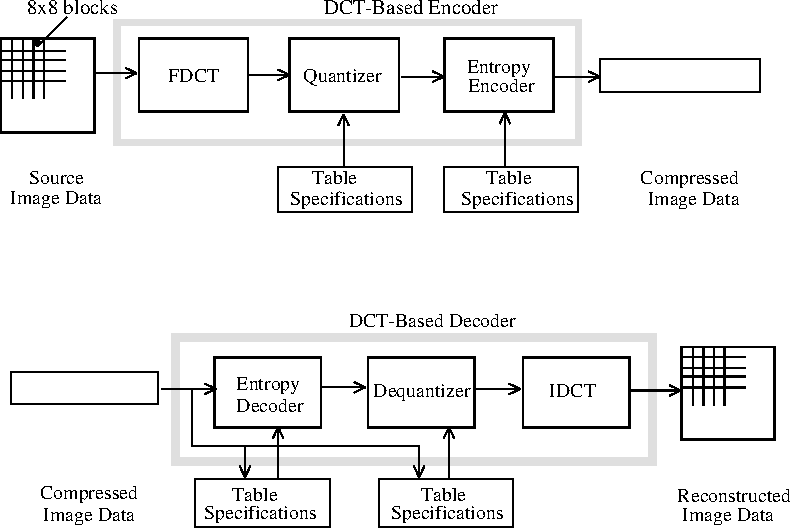
\includegraphics[width=0.75\textwidth]{figs/jpeg.pdf}
\caption{Diagrama geral que ilustra o funcionamento (codificação e decodificação) do método de compressão JPEG. Fonte:~\cite{jpeg}}
\end{figure} 
\end{frame}
%------------------------------------------------------
\begin{frame}
\frametitle{Transformada Discreta de Cosssenos (DCT)}
\begin{itemize}
\item Cada bloco 8x8 pode ser replicado por 64 (8x8) ondas de cossenos.
\item Analisa as frequências dos valores originais da imagem ao longo de cada linha e coluna usando um conjunto de ondas de cossenos oscilando em diferentes frequências e amplitudes. Cada bloco é representado usando estas ondas.
\end{itemize} 
\end{frame}
%------------------------------------------------------
\begin{frame}
\frametitle{Transformada Discreta de Cosssenos (DCT)}
\begin{figure}
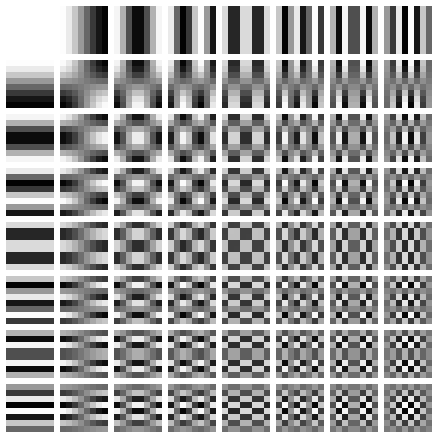
\includegraphics[width=0.48\textwidth]{figs/DCT-8x8.png}
\caption{64 ondas base de cossenos que produzem qualquer imagem 8x8. A DCT irá calcular os coeficientes - a contribuição de cada uma dessas ondas que somadas irão recriar a imagem perfeitamente. Fonte:~\cite{dct}}
\end{figure}
\end{frame}
%------------------------------------------------------
\newcommand\round[1]{\left[#1\right]}
\begin{frame}
\frametitle{Quantização}
\begin{itemize}
\item Para o \textit{encoder} será usada a seguinte equação:
\begin{equation}\round{F^Q(u,v) = \dfrac{F(u,v)}{Q(u,v)}}\end{equation}
\begin{enumerate}
\item Parte em que há maior perda de informação da imagem.
\item Cada um dos 64 coeficientes DCT $F(u,v)$ são uniformemente quantizados em conjunto com uma tabela de quantização de 64 elementos, que é definida pelo nível de qualidade escolhido para a aplicação.
\item Remove altas frequências definindo altos valores para $Q(u,v)$ (passo de quantização)
\end{enumerate}
\item No final, para cada bloco 8 por 8 da imagem original, existirá uma matriz quantizada.
\end{itemize}
\end{frame}
%------------------------------------------------------
\begin{frame}
\frametitle{Codificação}
\begin{figure}
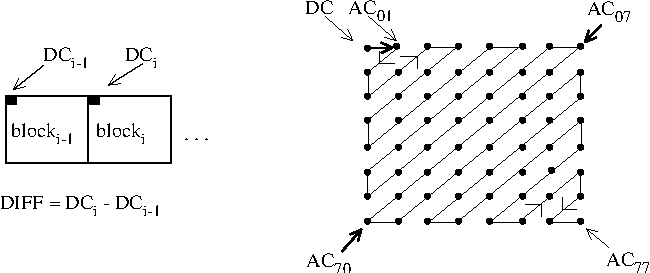
\includegraphics[width=\textwidth]{figs/coding_jpeg.pdf}
\caption{Codificação dos Direct Current (DC) coeficientes (esquerda) e sequência zig-zag usada para codificar todos os coeficientes (direita). Fonte:~\cite{jpeg}}
\end{figure}
\end{frame}
%------------------------------------------------------
\subsection{Redes Neurais}
%------------------------------------------------------
\begin{frame}
\frametitle{Aprendizado Profundo}
\begin{itemize}
\item Para muitas tarefas em inteligência artificial, é necessário extrair \textit{features} (características) dos dados.
\begin{enumerate}
\item As vezes é difícil saber quais \textit{features} devem ser extraídas.
\item Solução: aprender a representação dos dados (\textit{representation learning}).
\end{enumerate}
\item \textit{Deep learning} resolve o problema de \textit{representation learning} introduzindo representações que são expressadas em termos de outras representações mais simples.
\item Por exemplo, redes reurais convolucionais são capaz de capturar dependências espaciais e temporais na imagem ao aplicar filtros.
\end{itemize} 
\end{frame}
%------------------------------------------------------
\subsection{Autoencoders}
%------------------------------------------------------
\begin{frame}
\frametitle{Autoencoder}
\begin{figure}
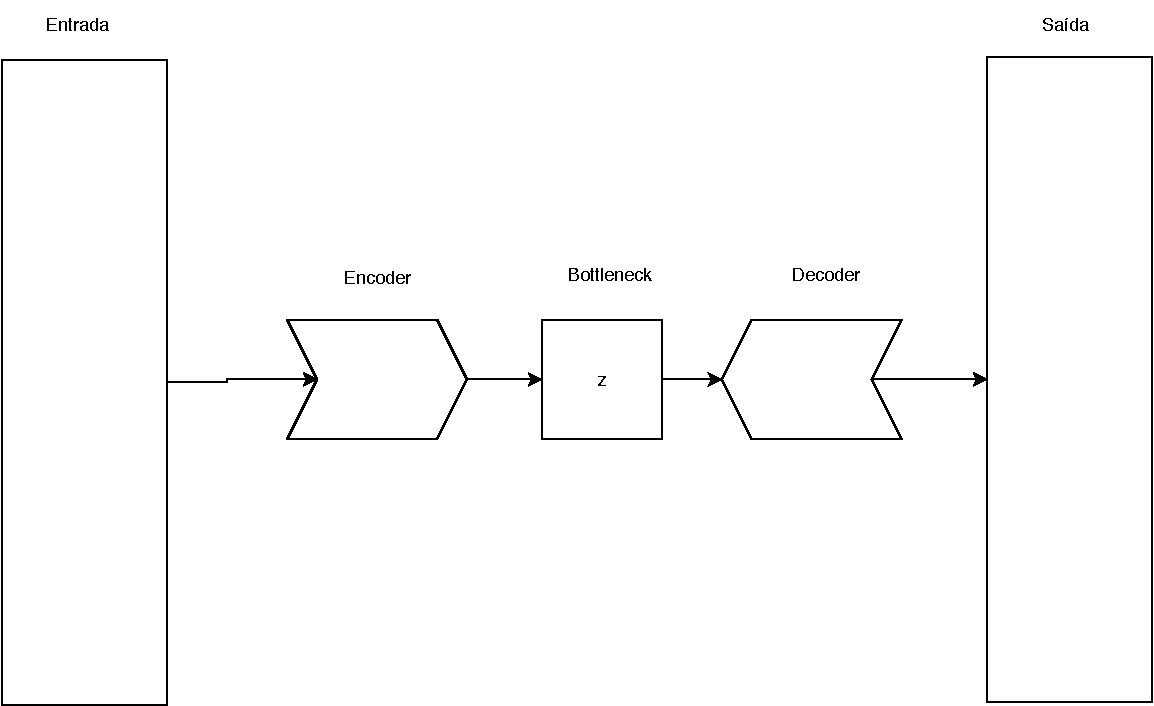
\includegraphics[width=0.8\textwidth]{figs/autoencoder.pdf}
\caption{Ilustração de um \textit{autoencoder}, uma técnica de aprendizado não supervisionado na qual pode-se utilizar redes neurais para a tarefa de aprendizado de representações.}
\end{figure}
\end{frame}
%------------------------------------------------------
\begin{frame}
\frametitle{Autoencoder para Compressão de imagens}
\begin{itemize}
\item Usa-se um binarizador na camada de gargalo para transformar os valores em ponto flutuante para inteiros que serão binarizados.
\item Valores contínuos precisam ser quantizados para um conjunto finito de valores discretos.
\begin{enumerate}
\item Códigos práticos precisam ter entropia finita (variáveis aleatórias contínuas fazem com que o logaritmo seja ``infinito'').
\item Redução de espaço consumido pela código da imagem codificada.
\item Introdução de erro!
\end{enumerate}
\end{itemize}
\end{frame}
%------------------------------------------------------
\begin{frame}
\frametitle{Compressão de Imagens com Taxa Variável usando Redes Neurais Recorrentes~\cite{toderici}}
\begin{itemize}
\item Mostrou que é possível treinar uma única rede neural recorrente e alcançar melhores resultados do que o \textbf{JPEG} para uma determinada \textit{quality} e métrica visual.
\item Abordagem ponta a ponta (modelagem e codificação) para compressão de imagens.
\item Modelo pode ser sumarizado pelo seguinte conjunto de equações:
      $$b_t = B(E_t(r_{t-1})), \, \hat{\mathbf{x}}_t = D_t(b_t) + \gamma\hat{\mathbf{x}}_{t-1},$$
      $$r_t = \mathbf{x} - \hat{\mathbf{x}}_t, \, r_0 = \mathbf{x}, \, \hat{\mathbf{x}}_0 = 0$$
\end{itemize}
\end{frame}
%------------------------------------------------------
\begin{frame}
\frametitle{Binarizador}
\begin{itemize}
\item Função de binarização $b(x)$:
\begin{equation} b(\mathbf{x}) = \mathbf{x} + \epsilon \,\in \{-1, 1\},\, \epsilon \sim \begin{cases} 
1 - \mathbf{x}\, \text{ com probabilidade } \frac{1+\mathbf{x}}{2},\\
-1 - \mathbf{x}\, \text{ com probabilidade } \frac{1-\mathbf{x}}{2},\\
\end{cases} \end{equation}
\item Binarizador: \begin{equation} B(\mathbf{x}) = b(tanh(W\mathbf{x} + b)) \end{equation}
\item Essa função é aplicada somente na \textit{Forward pass}. Para a \textit{Backward pass} é usada a derivada da esperança.
\item Uma vez que a rede esteja treinada $b$ é substituída por:
\begin{equation}
b^{inf}(\mathbf{x}) = \begin{cases}
-1,\, \text{ se } \mathbf{x} < 0,\\
1,\, \text{ caso contrário. }\\
\end{cases}
\end{equation}
\end{itemize}
\end{frame}
%------------------------------------------------------
\begin{frame}
\frametitle{Ilustração do Modelo Recorrente}
\begin{figure}
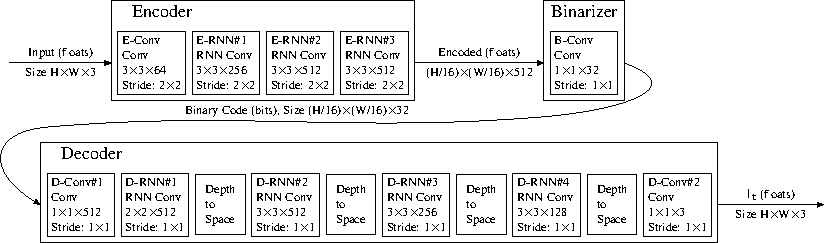
\includegraphics[width=\textwidth]{figs/toderici_4.pdf}
\caption{Autoencoder residual convolucional usando \textit{LSTM} convolucionais. As últimas linhas dos retângulos referentes aos blocos convolucionais denotam a largura do \textit{kernel}, altura do \textit{kernel} e a quantidade de filtros utilizada, respectivamente. \textit{Depth to Space} é uma operação de \textit{shuffle} dos pixels. Reproduzida de:~\cite{toderici2017}}
\label{fig:rec_conv_ae}
\end{figure}
\end{frame}
%------------------------------------------------------
\section{Metodologia}
%------------------------------------------------------
\subsection{Bases de Dados}
%------------------------------------------------------
\begin{frame}
\frametitle{Bases de Dados}
\begin{itemize}
\item Foram pegas imagens de \href{https://www.compression.cc/}{CLIC}, \href{https://data.vision.ee.ethz.ch/cvl/DIV2K/}{DIV2K} e \href{https://mmspg.epfl.ch/downloads/ultra-eye/}{EYE}.
\item Foram gerados 6,231,440 \textit{patches} com 32 pixels de largura e altura. Estes \textit{patches} foram divididos em 5 bases:
\begin{enumerate}
    \item \textbf{BD0}: formada por 1,248,978 de \textit{patches} que pertencem ao grupo dos 20\% com menor entropia;
    \item \textbf{BD1}: formada por 1,251,421 de \textit{patches} que pertencem ao grupo dos que estão na faixa 40\% à 60\% (porcentagem dada pelo \textit{patch} com maior entropia);
    \item \textbf{BD2}: formada por 1,248,725 de \textit{patches} que pertencem ao grupo dos 20\% com maior entropia;
    \item \textbf{BD3}: formada por 1,247,033 de \textit{patches} pegos de forma aleatória. Correspondem à 20\% do total.
    \item \textbf{BD4}: formada por 1,246,698 de \textit{patches}. 20\% do total retirados aleatoriamente dos 50\% de \textit{patches} com maior entropia.
\end{enumerate}
\end{itemize}
\end{frame}
%------------------------------------------------------
\begin{frame}
\frametitle{Bases de Dados}
\begin{figure}
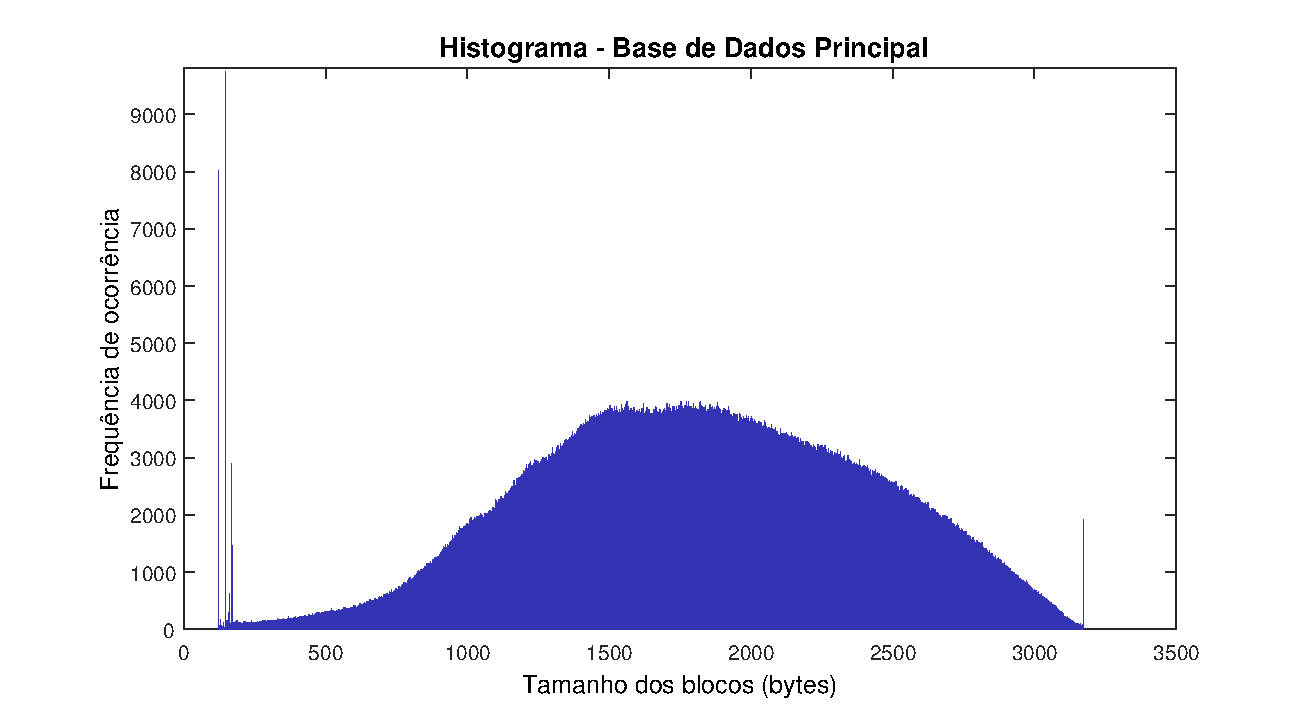
\includegraphics[width=\textwidth]{figs/hist.eps}
\caption{Histograma da base de dados completa.}
\end{figure}
\end{frame}
%------------------------------------------------------
\subsection{Modelos Desenvolvidos}
%------------------------------------------------------
\begin{frame}
\frametitle{Modelo 1}
\begin{figure}
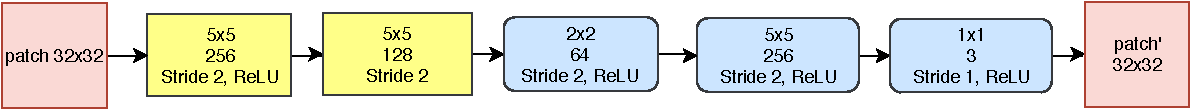
\includegraphics[width=\textwidth]{figs/conv_ae.pdf}
\caption{Ilustração do Modelo 1. Autoencoder sem binarizador com o objetivo de avaliar as bases de dados construídas. Treinado por 50,000 iterações.}
\end{figure}
\end{frame}

%------------------------------------------------------
\begin{frame}
\frametitle{Modelos 2 e 3}
\begin{itemize}
    \item Esses modelos seguem a arquitetura apresentada na \textbf{Figura}~\ref{fig:rec_conv_ae} com 6 níveis de resíduos. 
    \item Treinados nas bases \textbf{BD2} e \textbf{BD4} e testados na base Kodak~\cite{kodak}. 
    \item 150,000 iterações.
    \item A função de custo utilizada no Modelo 2 é a \textbf{MSE}. 
    \item Função de custo utilizada no Modelo 3: $$MSE + Ke^{(-0.07r)}Q,$$
    onde $K = 3.5 \times 10^{-7}$ $Q$ é a quantidade de bits 1 no latente binarizado e $r \in \{1, \cdots 6\}$ é o nível de resíduo. 
\end{itemize}
\end{frame}

%------------------------------------------------------
\begin{frame}
\frametitle{Modelo 4}
\begin{itemize}
    \item Foram usadas as bases \textbf{BD2}, \textbf{BD3} e \textbf{BD4} como treino. 
    \item 500,000 iterações.
    \item Testado em imagens das bases Kodak~\cite{kodak} e Clic~\cite{clic}.
    \item 10 níveis de resíduos.
\end{itemize}
\end{frame}
%------------------------------------------------------
\section{Experimentos}
%------------------------------------------------------
\subsection{JPEG}
%------------------------------------------------------
\begin{frame}
\frametitle{Desempenho JPEG}
\begin{table}[]
\caption{Tabela contendo médias obtidas pelo \textbf{JPEG} em cada uma das bases de teste utilizadas}
\begin{tabular}{|l|l|l|l|l|l|}
\hline
\textbf{Bases}                                                                   & \textbf{Taxa (BPP)} & \textbf{PSNR} & \textbf{SSIM} & \textbf{MSSIM} & \textbf{Quality} \\ \hline
\textbf{\begin{tabular}[c]{@{}l@{}}CLIC Mobile test\\ (patches 32)\end{tabular}} & 8            & 44.23         & 0.98          & 0.99           & 94.06            \\ \hline
\textbf{CLIC Mobile test}                                                        & 2            & 39.58         & 0.96          & 0.99           & 88.69            \\ \hline
\textbf{Kodak}                                                                   & 2            & 36.77         & 0.95          & 0.99           & 85.91            \\ \hline
\textbf{BD0}                                                                     & 8            & 57.85         & 0.99          & 0.99           & 99.18            \\ \hline
\textbf{BD1}                                                                     & 8            & 42.94         & 0.97          & 0.99           & 95.94            \\ \hline
\textbf{BD2}                                                                     & 8            & 32.31         & 0.95          & 0.99           & 83.69            \\ \hline
\textbf{BD3}                                                                     & 8            & 43.84         & 0.96          & 0.99           & 93.94            \\ \hline
\textbf{BD4}                                                                     & 8            & 36.72         & 0.96          & 0.99           & 89.68            \\ \hline
\end{tabular}
\end{table}
\end{frame}
%------------------------------------------------------
\subsection{Modelo 1}
%------------------------------------------------------
\begin{frame}
\frametitle{Treino e Teste em todas as bases para o Modelo 1}
\begin{table}
\caption{Tabela contendo o valor da \textit{PSNR}, em decíbeis, dos testes do \textbf{Modelo 1} com o uso do otimizador \textit{Adam} e \textit{learning rate} fixa. As linhas denotam a base de treino utilizada. As colunas denotam as bases de teste usadas para avaliação do modelo. O índice ``todas'' se refere ao uso de todas as imagens de todas as bases \textbf{BD} para treino}
\begin{tabular}{|l|l|l|l|l|l|}
\hline
\textbf{\begin{tabular}[c]{@{}l@{}}Treino (linhas) x \\Teste (colunas)\end{tabular}} & \textbf{BD0}   & \textbf{BD1}   & \textbf{BD2}   & \textbf{BD3}   & \textbf{BD4}   \\ \hline
\textbf{BD0}                                                                          & 49.66          & 38.07          & 26.34          & 38.05          & 31.13          \\ \hline
\textbf{BD1}                                                                          & 47.57          & 44.08          & 34.54          & 42.66          & 38.69          \\ \hline
\textbf{BD2}                                                                          & \textbf{53.69} & \textbf{51.16} & \textbf{44.07} & \textbf{50.06} & \textbf{47.14} \\ \hline
\textbf{BD3}                                                                          & 50.62          & 47.88          & 39.76          & 46.59          & 43.25          \\ \hline
\textbf{BD4}                                                                          & 47.30          & 46.98          & 41.10          & 45.63          & 43.75          \\ \hline
\textbf{Todas}                                                                        & 46.77          & 46.35          & 43.94          & 45.88          & 45.08          \\ \hline
\end{tabular}
\end{table}
\end{frame}
%------------------------------------------------------
\subsection{Modelos 2 e 3}
%------------------------------------------------------
\begin{frame}
\frametitle{Resultados dos Modelos 2 e 3}
\begin{table}
\caption{Média obtida pelos Modelos 2 e 3. Foi utilizado \textit{10-fold cross validation} para obter estes resultados.}
\begin{tabular}{|l|l|l|l|}
\hline
Modelos  & Taxa (BPP) & PSNR (dB) & SSIM    \\ \hline
Modelo 2 & 0.71       & 30.23     & 0.86340 \\ \hline
Modelo 3 & 0.71       & 30.31     & 0.86498 \\ \hline
\end{tabular}
\end{table}

\begin{figure}
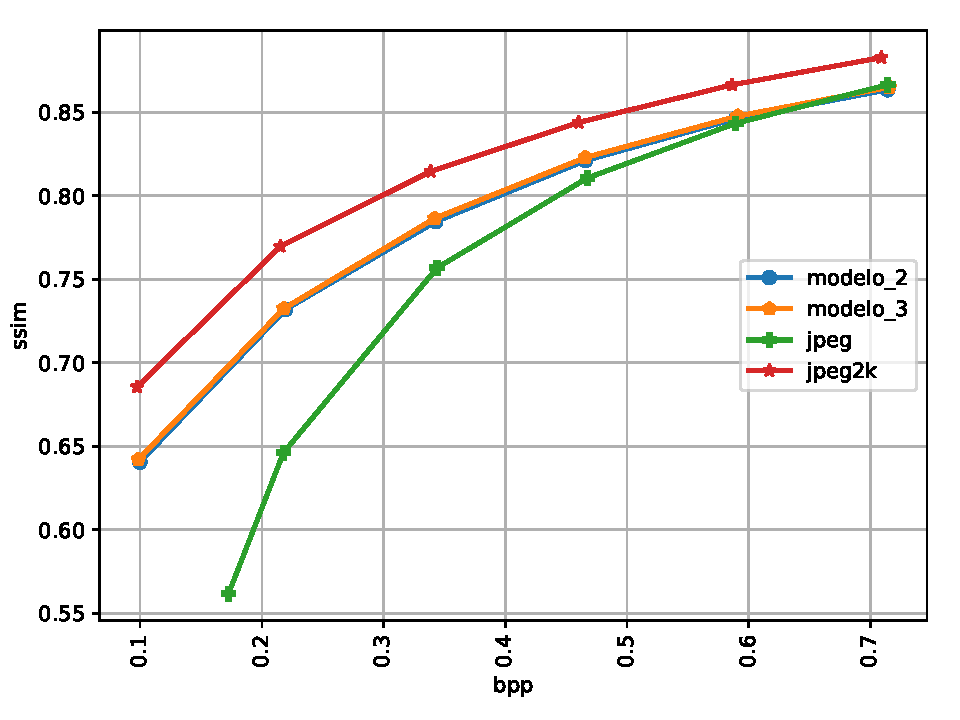
\includegraphics[width=0.4\textwidth]{figs/_mean_plot_loss_ssim.pdf}
\caption{Comparação dos Modelos 2 e 3 para a métrica SSIM}
\end{figure}
\end{frame}
%------------------------------------------------------
\subsection{Modelo 4}
%------------------------------------------------------
\begin{frame}
\frametitle{Resultados do Modelo 4 para a Base Kodak~\cite{kodak}}
\begin{figure}
\centering
\begin{subfigure}{.5\textwidth}
  \centering
  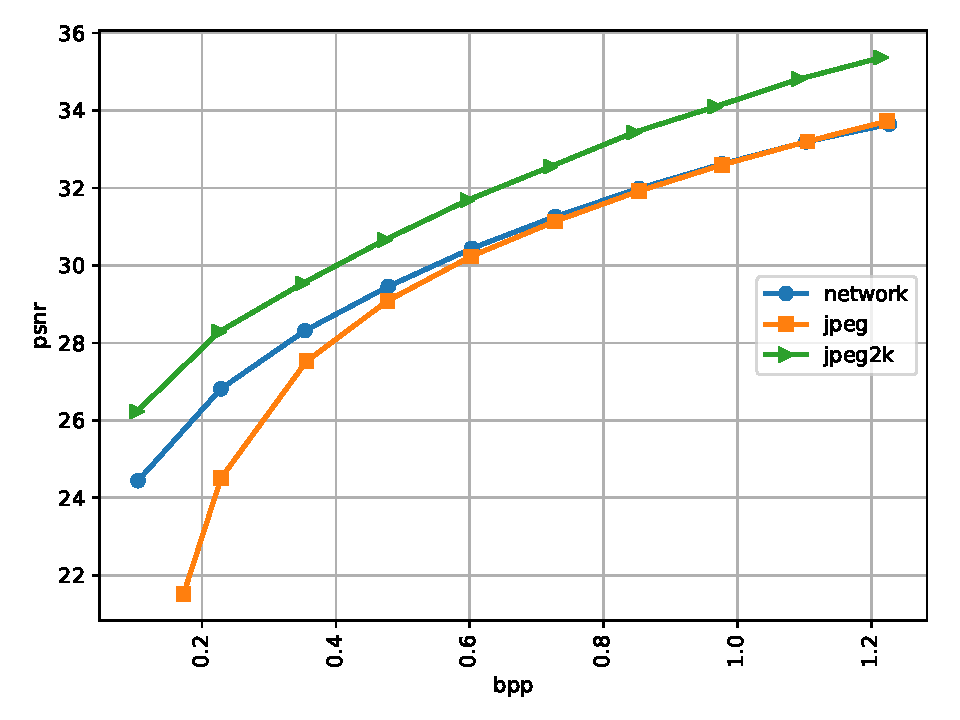
\includegraphics[width=.8\textwidth]{figs/_mean_plot_psnr_10levels.pdf}
  \caption{Modelo 4 na métrica PSNR}
  \label{fig:mod4_1:sub1}
\end{subfigure}%
\begin{subfigure}{.5\textwidth}
  \centering
  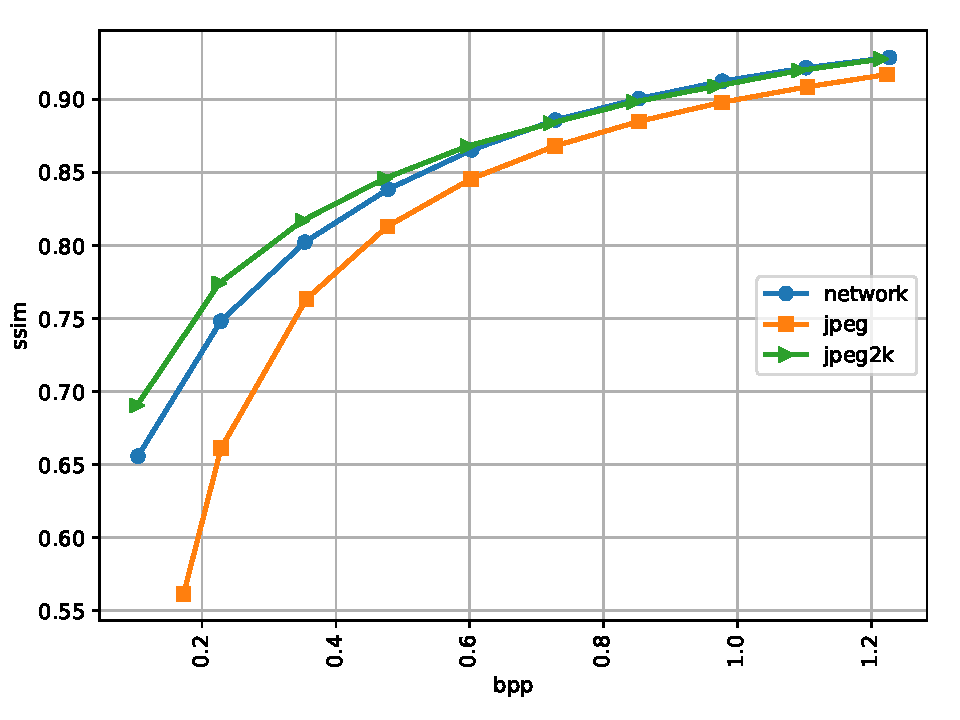
\includegraphics[width=.8\textwidth]{figs/_mean_plot_ssim_10levels.pdf}
  \caption{Modelo 4 na métrica SSIM}
  \label{fig:mod4_1:sub2}
\end{subfigure}
\caption{Modelo superou o \textbf{JPEG} nas métricas \textit{SSIM} e \textit{MS-SSIM} e o \textbf{JPEG2000} na métrica \textit{SSIM}}
\label{fig:mod4_1}
\end{figure}
\end{frame}
%------------------------------------------------------
\begin{frame}
\frametitle{Resultados do Modelo 4 para 47 imagens com muito conteúdo de alta frequência retiradas de~\cite{kodak} e~\cite{clic}}
\begin{figure}
\centering
\begin{subfigure}{.5\textwidth}
  \centering
  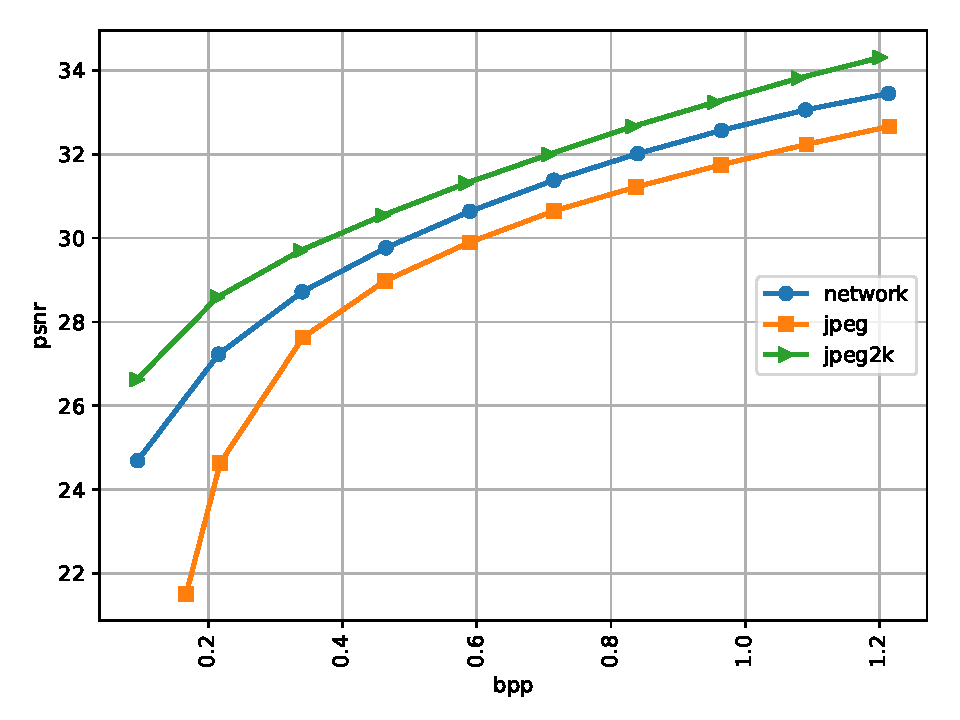
\includegraphics[width=.8\textwidth]{figs/_mean_plot_psnr_hf_10levels.pdf}
  \caption{Modelo 4 na métrica PSNR}
  \label{fig:mod4_2:sub1}
\end{subfigure}%
\begin{subfigure}{.5\textwidth}
  \centering
  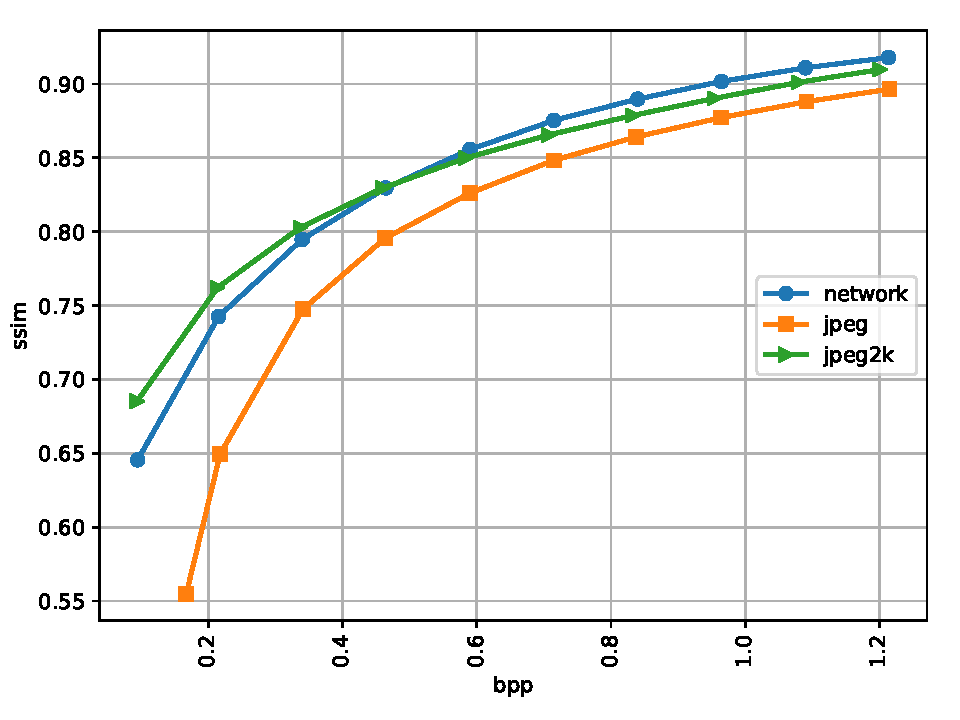
\includegraphics[width=.8\textwidth]{figs/_mean_plot_ssim_hf_10levels.pdf}
  \caption{Modelo 4 na métrica SSIM}
  \label{fig:mod4_2:sub2}
\end{subfigure}
\caption{Modelo superou o \textbf{JPEG} nas métricas \textit{SSIM}, \textit{PSNR} e \textit{MS-SSIM} e o \textbf{JPEG2000} na métricas \textit{SSIM} e \textit{MS-SSIM}}
\label{fig:mod4_2}
\end{figure}
\end{frame}
%------------------------------------------------------
\begin{frame}
\frametitle{Imagens com muito conteúdo de alta frequência retiradas de~\cite{clic} e~\cite{kodak}}
\begin{figure}
\centering
\begin{subfigure}{.5\textwidth}
  \centering
  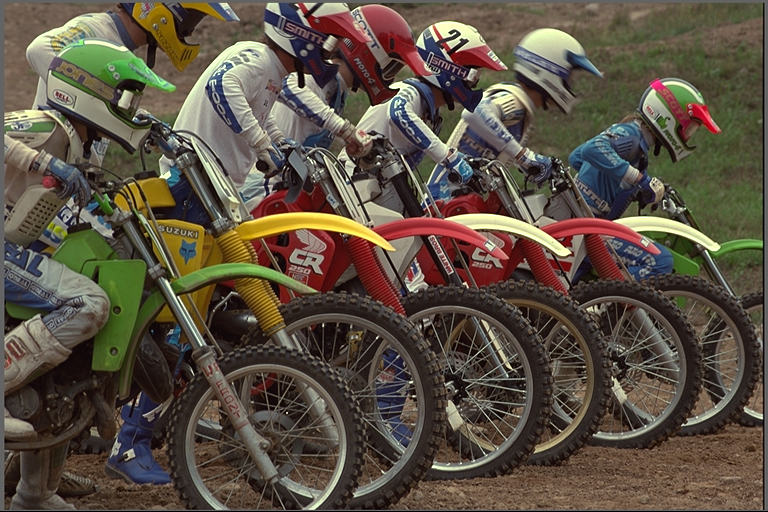
\includegraphics[width=0.7\textwidth]{figs/kodim05.png}
  \caption{Resultados do Modelo 4 para a métrica PSNR}
  \label{fig:figs:sub1}
\end{subfigure}%
\begin{subfigure}{.5\textwidth}
    \centering
    \includegraphics[width=0.8\textwidth]{figs/jason-leem-143987.png}
    \caption{Imagem \textit{jason-leem} retirada de~\cite{clic}}
    \label{fig:figs:sub2}
\end{subfigure}
\caption{Imagens com muito conteúdo de alta frequência}
\end{figure}
\end{frame}
%------------------------------------------------------
\begin{frame}
\frametitle{Resultados do Modelo 4 para a imagem~\ref{fig:figs:sub1}}
\begin{figure}
\centering
\begin{subfigure}{.5\textwidth}
  \centering
  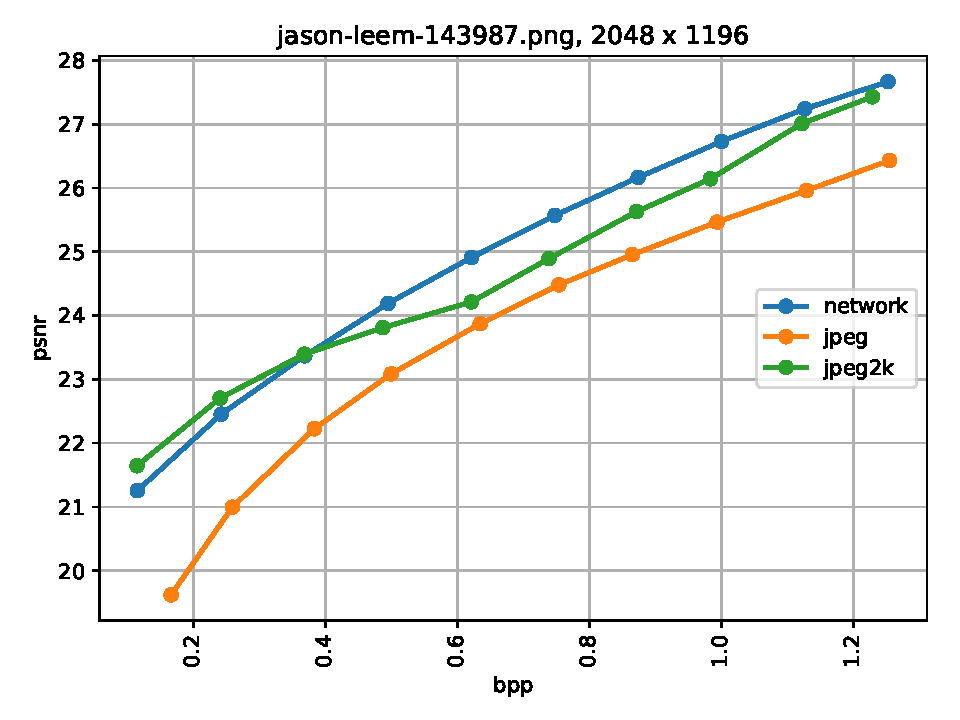
\includegraphics[width=0.9\textwidth]{figs/jason-leem-143987_plot_psnr.pdf}
  \caption{Resultados do Modelo 4 para a métrica PSNR}
  \label{fig:mod4_3:sub1}
\end{subfigure}%
\begin{subfigure}{.5\textwidth}
  \centering
  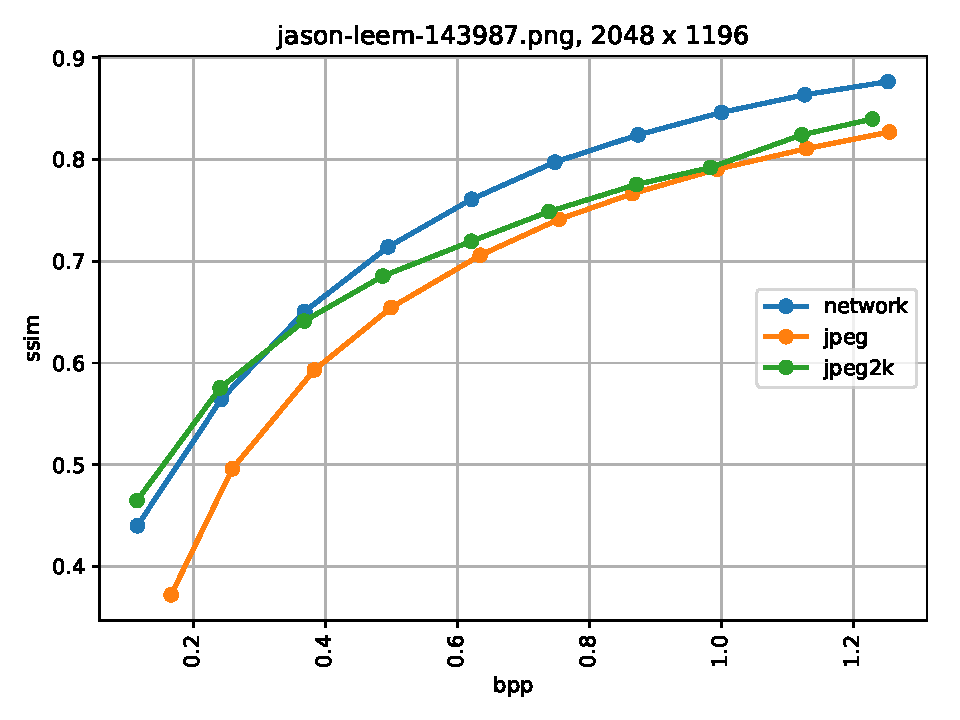
\includegraphics[width=0.9\textwidth]{figs/jason-leem-143987_plot_ssim.pdf}
  \caption{Resultados do Modelo 4 para a métrica SSIM}
  \label{fig:mod4_3:sub2}
\end{subfigure}
\caption{Pode-se perceber que o Modelo 4 superou ambos os codecs para ambas as métricas. }
\label{fig:mod4_3}
\end{figure}
\end{frame}
%------------------------------------------------------
\begin{frame}
\frametitle{Resultados do Modelo 4 para a imagem~\ref{fig:figs:sub2}}
\begin{figure}
\centering
\begin{subfigure}{.5\textwidth}
  \centering
  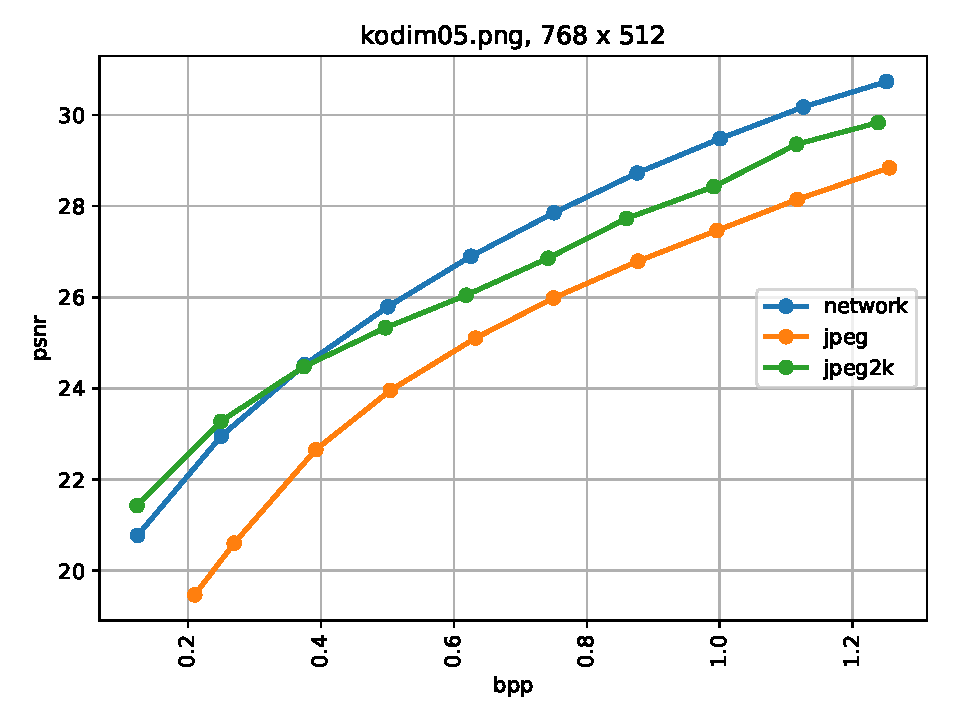
\includegraphics[width=0.9\textwidth]{figs/kodim05_plot_psnr.pdf}
  \caption{Resultados do Modelo 4 para a métrica PSNR}
  \label{fig:mod4_4:sub1}
\end{subfigure}%
\begin{subfigure}{.5\textwidth}
  \centering
  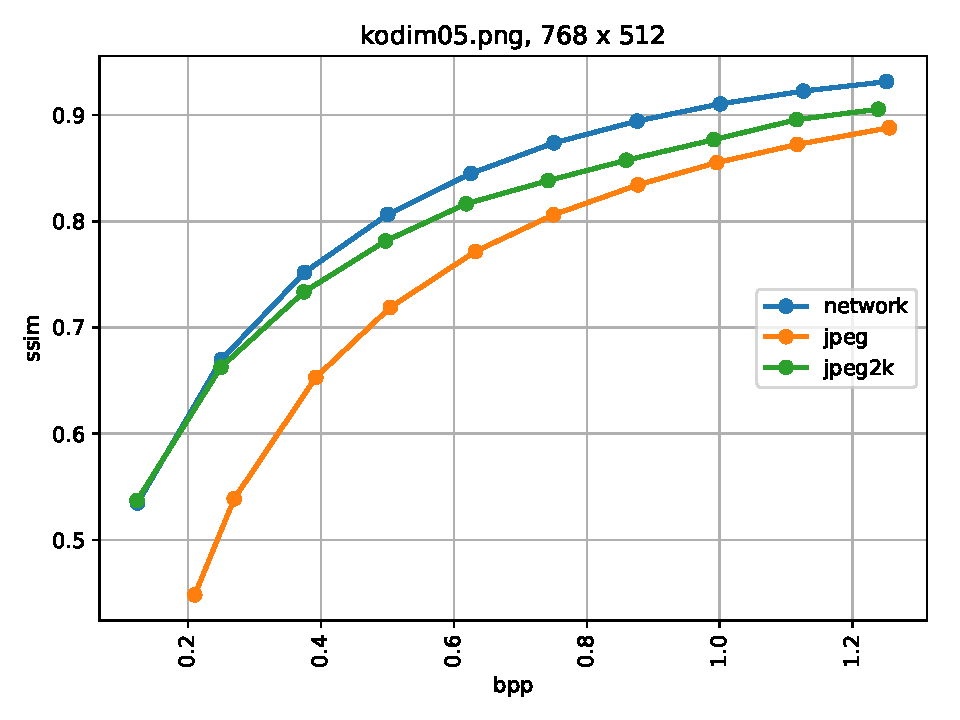
\includegraphics[width=0.9\textwidth]{figs/kodim05_plot_ssim.pdf}
  \caption{Resultados do Modelo 4 para a métrica SSIM}
  \label{fig:mod4_4:sub2}
\end{subfigure}
\caption{Pode-se perceber que o Modelo 4 superou ambos os codecs para ambas as métricas. }
\label{fig:mod4_4}
\end{figure}
\end{frame}
%------------------------------------------------------
\begin{frame}
\frametitle{Reconstrução do Modelo 4 e dos codecs clássicos}
\begin{figure}
    \centering
    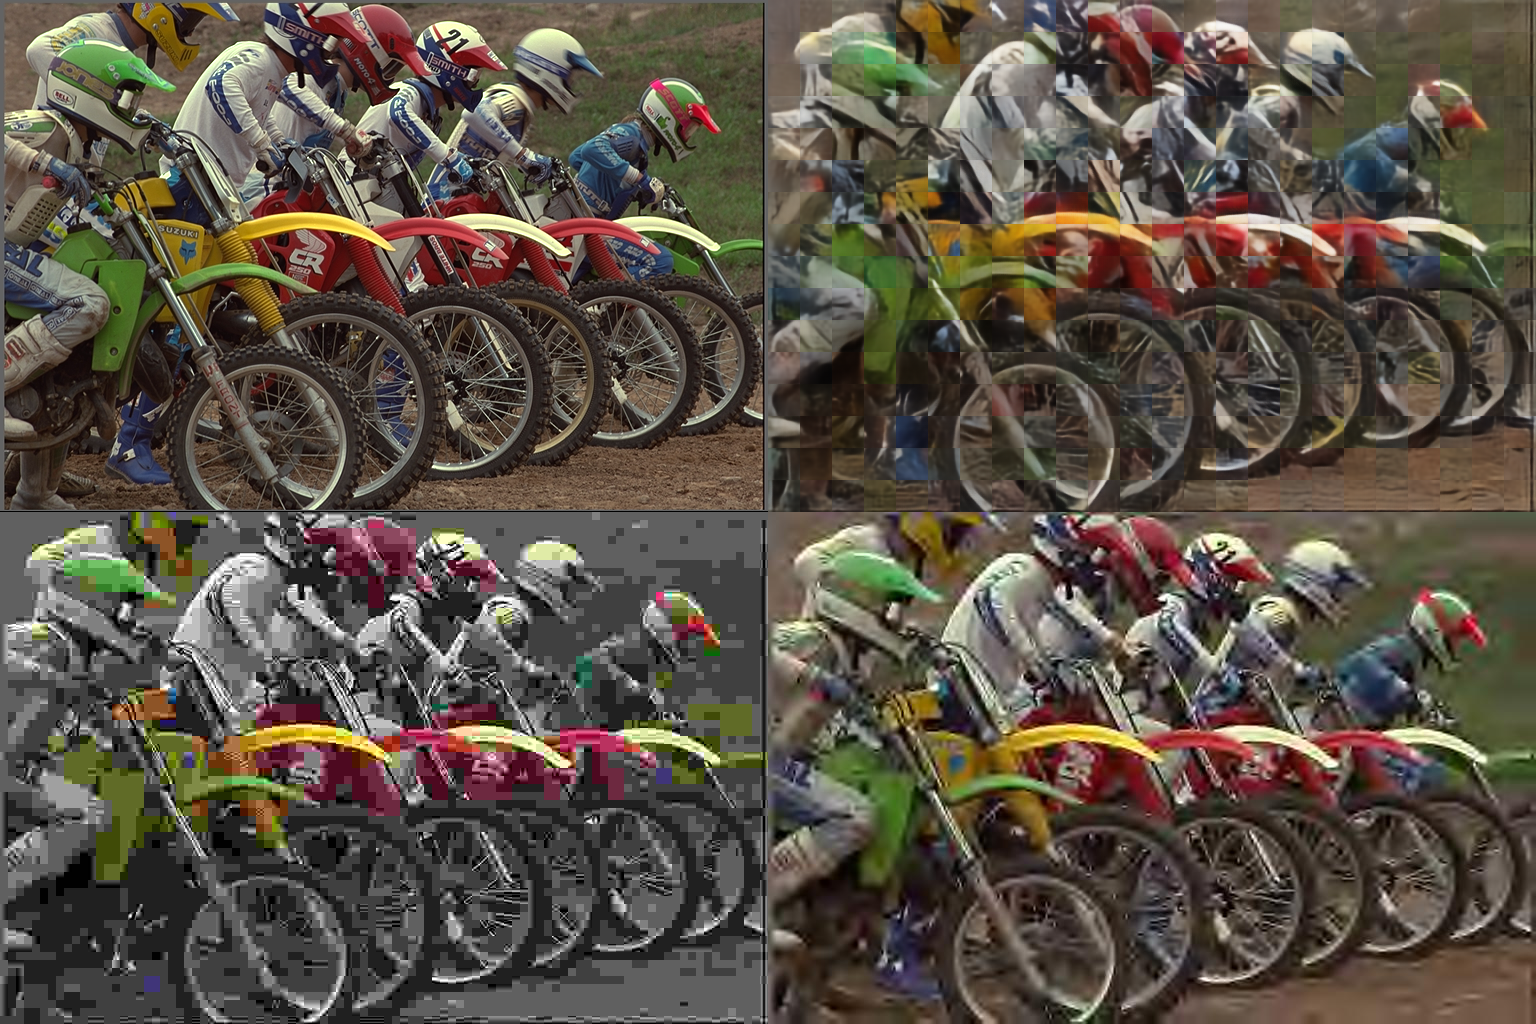
\includegraphics[width=0.7\textwidth]{figs/comparison_kodim05_0.png}
    \caption{Figura original (canto superior esquerdo), reconstruídas pelo modelo 4 (canto superior direito) a uma taxa de 0.12 bits por pixel, pelo JPEG (canto inferior esquerdo) a uma taxa de 0.21 bits por pixel e pelo JPEG2000 (canto inferior direito) a uma taxa de 0.12 bits por pixel. }
    \label{fig:mod4:kodim05:0}
\end{figure}
\end{frame}
%------------------------------------------------------
\begin{frame}
\frametitle{Reconstrução do Modelo 4 e dos codecs clássicos}
\begin{figure}
    \centering
    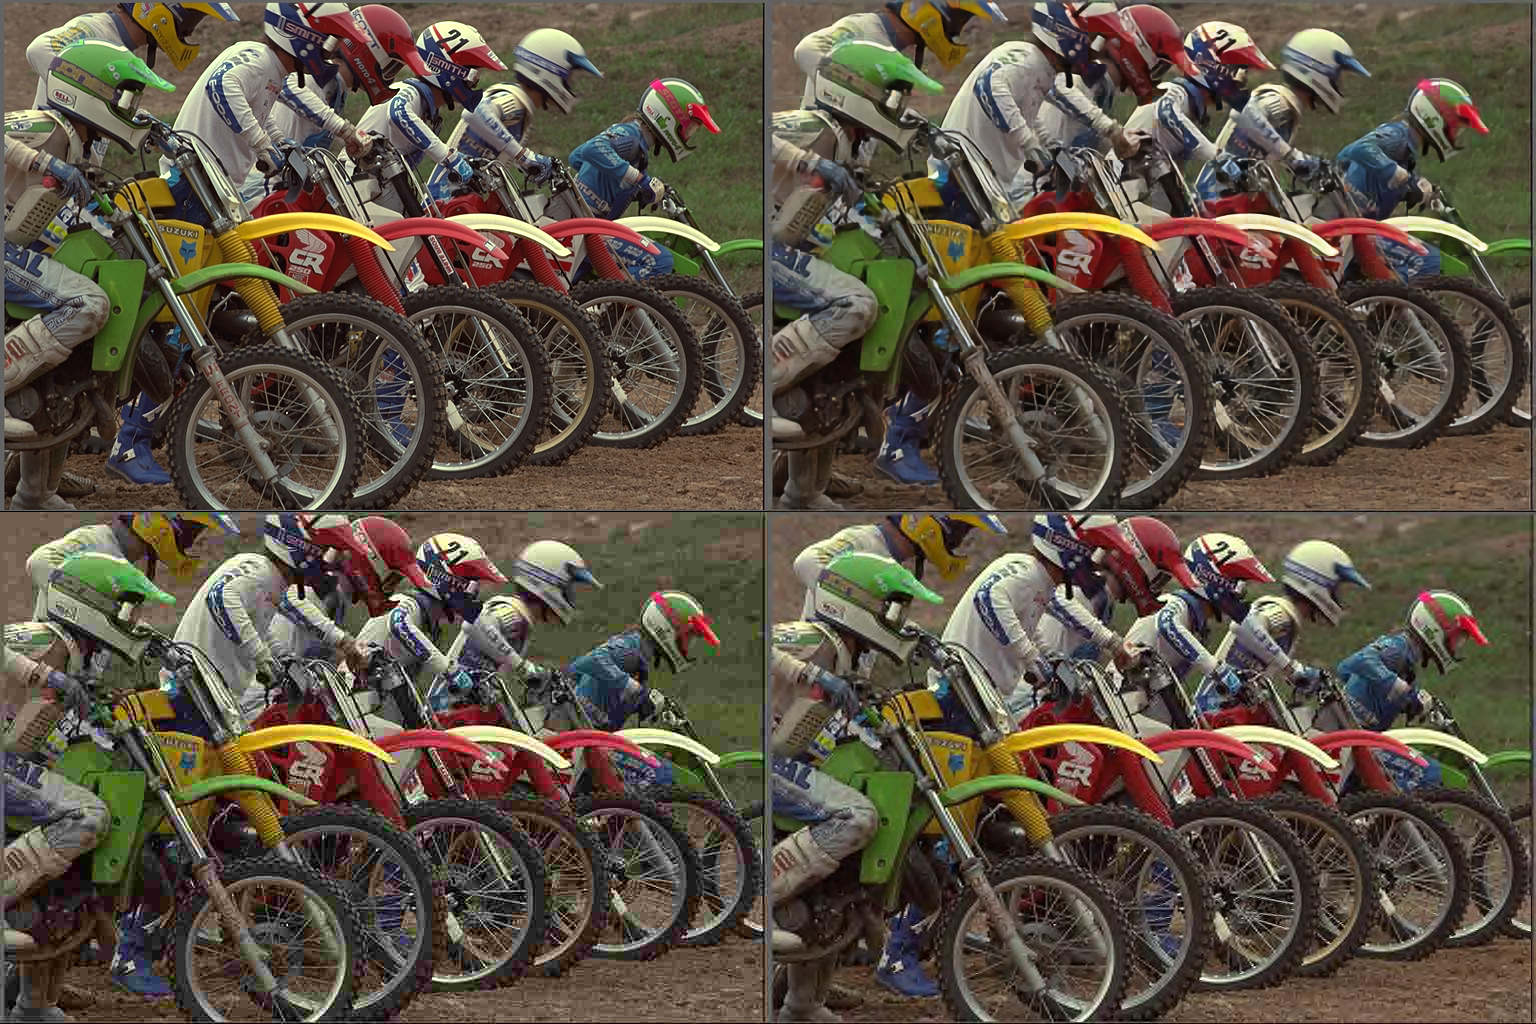
\includegraphics[width=0.7\textwidth]{figs/comparison_kodim05_3.png}
    \caption{Figura original (canto superior esquerdo), reconstruídas pelo modelo 4 (canto superior direito) a uma taxa de 0.47 bits por pixel, pelo JPEG (canto inferior esquerdo) a uma taxa de 0.50 bits por pixel e pelo JPEG2000 (canto inferior direito) a uma taxa de 0.50 bits por pixel. }
    \label{fig:mod4:kodim05:3}
\end{figure}
\end{frame}
%------------------------------------------------------
\subsection{Ganhos obtidos pelo GZIP}
%------------------------------------------------------
\begin{frame}
\frametitle{Média para a base dos Modelos 2, 3 e 4 Kodak~\cite{kodak}}
\begin{figure}
\begin{subfigure}{.5\textwidth}
    \centering
    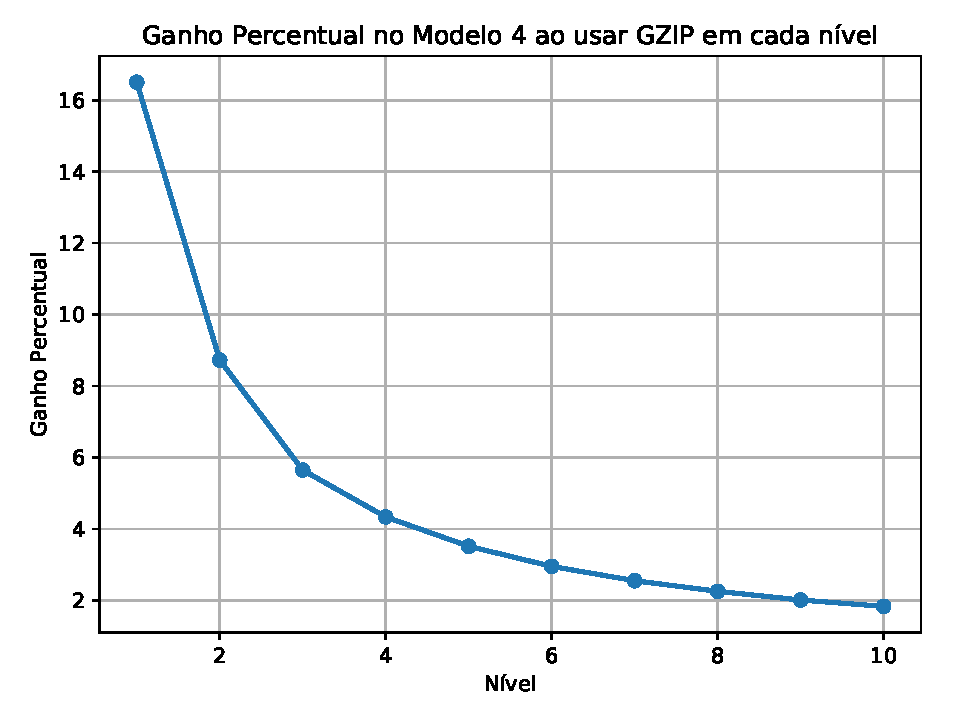
\includegraphics[width=0.8\textwidth]{figs/gain_gzip_mod4.pdf}
    \caption{Ganho percentual médio na taxa por nível de resíduo ao usar o codificador de entropia gzip nos bitstreams, gerados pelo Modelo 4, de cada nível para a base Kodak~\cite{kodak}}
\end{subfigure}%
\begin{subfigure}{.5\textwidth}
  \centering
  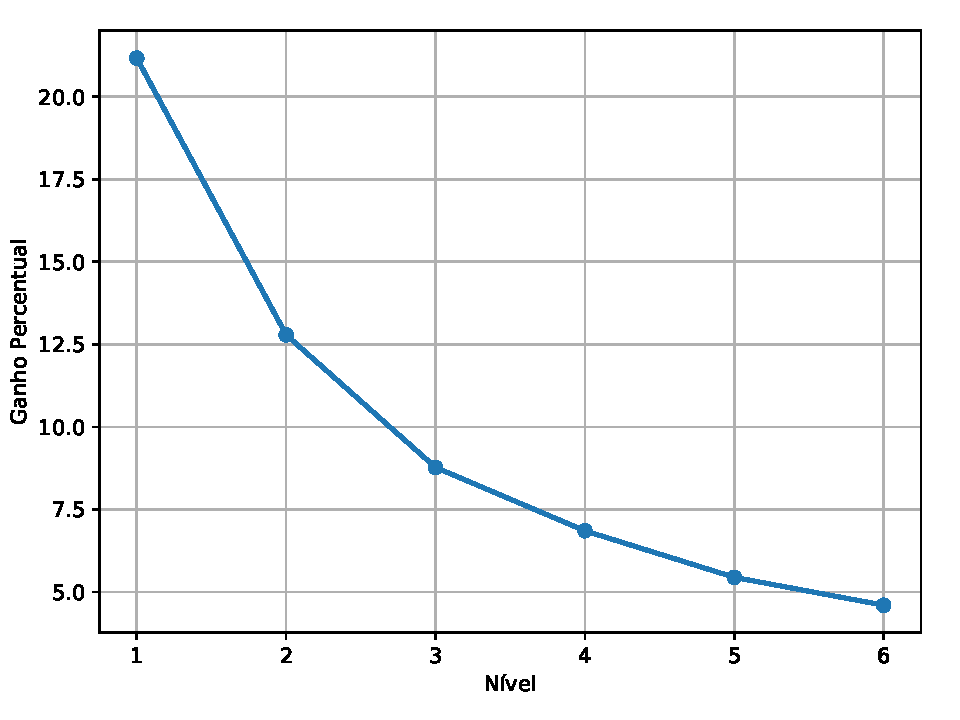
\includegraphics[width=0.8\textwidth]{figs/plot_gzip_model.pdf}
  \caption{Ganho percentual médio na taxa por nível de resíduo ao usar o codificador de entropia gzip nos bitstreams, gerados pelos Modelo 2 e 3, de cada nível para a base Kodak~\cite{kodak}}
\end{subfigure}
\end{figure}
\end{frame}
%------------------------------------------------------
\begin{frame}
\frametitle{Ganho por nível para a Imagem~\ref{fig:figs:sub2}}
\begin{figure}
    \centering
    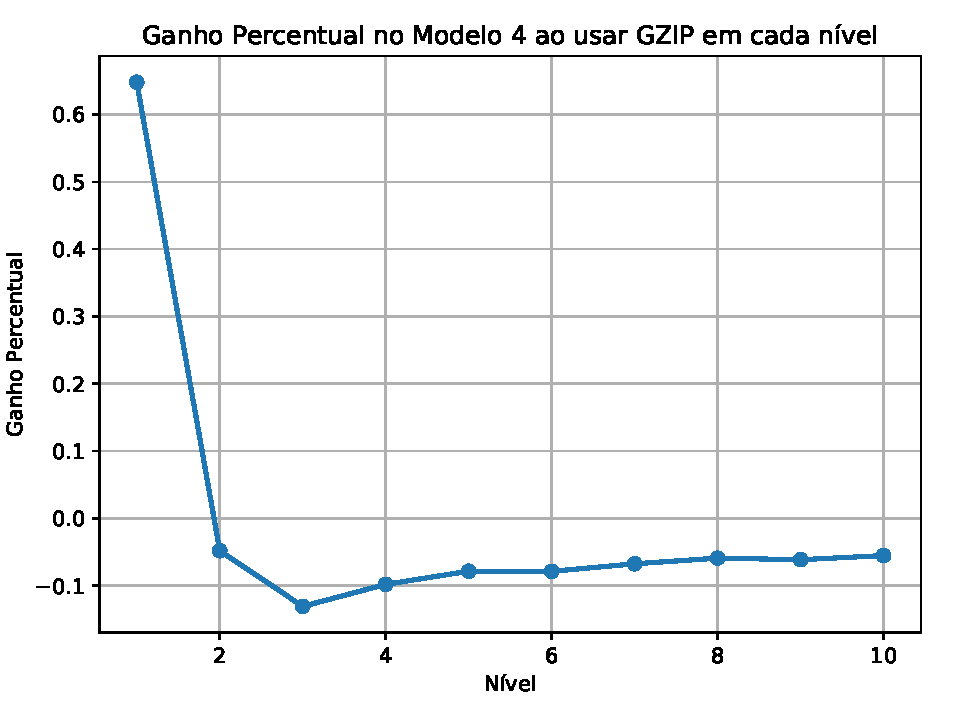
\includegraphics[width=0.7\textwidth]{figs/gain_gzip_kodim05.pdf}
    \caption{Ganho percentual médio na taxa por nível de resíduo ao usar o codificador de entropia nos bitstreams de cada nível para a Imagem~\ref{fig:figs:sub2}}
\end{figure}
\end{frame}
%------------------------------------------------------
\begin{frame}
\frametitle{Ganho por nível para Kodim20~\cite{kodak}}
\begin{figure}
\begin{subfigure}{.5\textwidth}
    \centering
    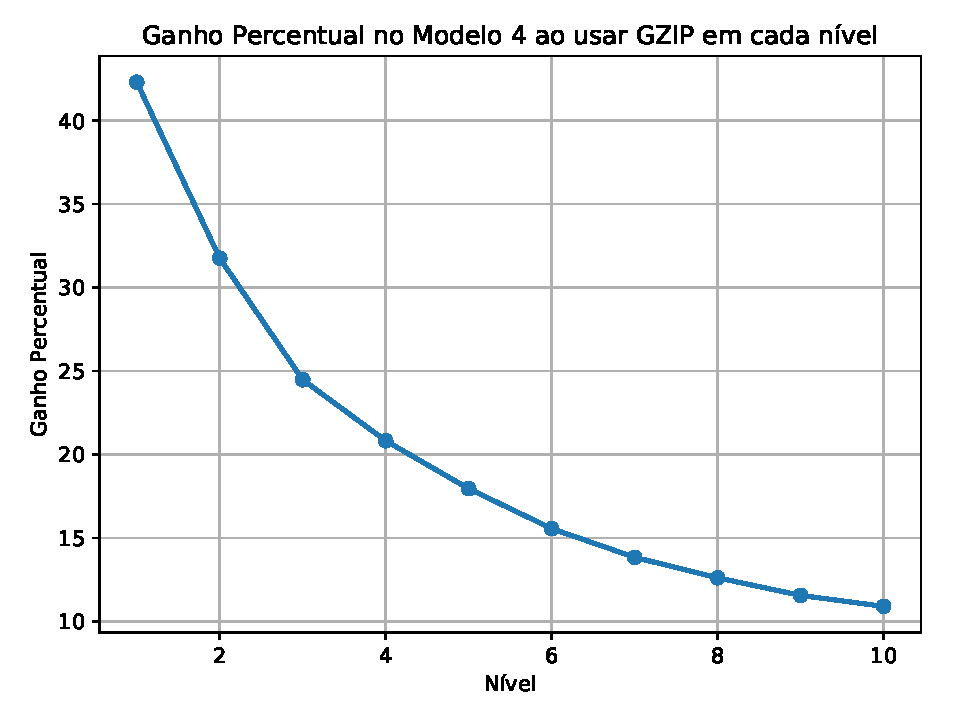
\includegraphics[width=0.8\textwidth]{figs/gain_gzip_kodim20.pdf}
    \caption{Ganho percentual na taxa por nível de resíduo ao usar o codificador de entropia gzip nos bitstreams, gerados pelo Modelo 4, de cada nível para a Imagem~\ref{fig:kodim20}}
\end{subfigure}%
\begin{subfigure}{.5\textwidth}
  \centering
  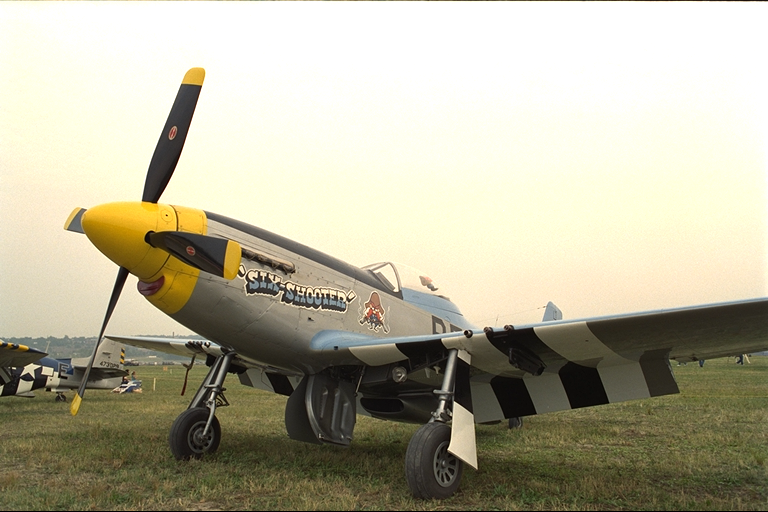
\includegraphics[width=0.8\textwidth]{figs/kodim20.png}
  \caption{Imagem Kodim20 da base Kodak~\cite{kodak}}
  \label{fig:kodim20}
\end{subfigure}
\end{figure}
\end{frame}
%------------------------------------------------------
\section{Conclusão}
%----------------------
\begin{frame}
\frametitle{Limitações do Trabalho}
\begin{itemize}
\item Custo computacional superior aos codecs clássicos.
\item Algoritmos flexíveis, porém quantização é uma operação não diferenciável o que dificulta treinamento de redes neurais.
\end{itemize}
\end{frame}
%------------------------------------------------
\begin{frame}
\frametitle{Análise e Perspectivas Futuras}
\begin{itemize}
    \item Modelos baseados em redes neurais conseguem superar os codecs clássicos em baixas taxas para imagens com muito conteúdo de alta frequência; 
    \item GZIP não comprime muito após a primeira iteração;
    \item Há um impacto significativo ao usar com muito conteúdo de alta frequência para treino do modelo;
    \item Impacto razoável com o uso de diferentes funções de custo. Bom espaço para ser explorado;
    \item Modelos apresentados são flexíveis para serem aplicados em outros tipos de mídia;
    \item Mesma quantidade de bits para todos os patches, o que não é uma boa abordagem do ponto de vista de compressão;
\end{itemize}
\end{frame}
%------------------------------------------------

%----------------------------------------------------
%----------------------------------------------------
\begin{frame}[allowframebreaks]
\frametitle{References}
\footnotesize{
\begin{thebibliography}{99} % Beamer does not support BibTeX so references must be inserted manually as below
%----------------------------------------------------
\bibitem[Sayood et al. 2017]{book_compression} Khalid Sayood
\newblock Introduction to Data Compression
\newblock Morgan Kaufmann

\bibitem[G. K. Wallace et al. 1993]{jpeg} Gregory K. Wallace
\newblock The JPEG Still Picture Compression Stantard
\newblock In: IEEE Transactions on Consumer Electronics

\bibitem[C. {Christopoulos} et al. 2000]{jpeg2000} C. Christopoulos and A. Skodras and T. Ebrahimi
\newblock The JPEG2000 Still Image Coding System: An Overview
\newblock In: IEEE Transactions on Consumer Electronics

\bibitem[Bellard et al. 2019]{bpg} Fabrice Bellard
\newblock BPG image format
\newblock In: \href{https://bellard.org/bpg/}{BPG}

\bibitem[Google 2019]{webp} WebP
\newblock Compression Techniques 
\newblock In: \href{https://developers.google.com/speed/webp/docs/compression}{Compression}

\bibitem[Nielsen et al. 2015]{nn_book} Michael A. Nielsen
\newblock Neural Networks and Deep Learning
\newblock In: \href{http://neuralnetworksanddeeplearning.com/}{Determination Press}

\bibitem[Goodfellow et al. 2015]{dl_book} Ian Goodfellow and Yoshua Bengio and Aaron Courville
\newblock Deep Learning
\newblock In: \href{http://www.deeplearningbook.org}{MIT Press}

\bibitem[Wikimedia Commons 2015]{dct} Wikimedia Commons
\newblock Wikimedia Commons, The Free Media Repository
\newblock In: \href{https://commons.wikimedia.org/w/index.php?curid=10414002}{DCT Figure}

\bibitem[Leslie et. al 2017]{clr} Leslie N. Smith
\newblock Cyclical Learning Rates for Training Neural Networks
\newblock In: Proceedings - IEEE Winter Conference on Applications of Computer Vision

\bibitem[Brad Kenstler et al. 2015]{exp} Brad Kenstler
\newblock Cyclical Learning Rate (CLR)
\newblock In: \href{https://github.com/bckenstler/CLR/}{GitHub Repository}

\bibitem[CS231n Course Materials 2019]{cnn} CS231n
\newblock CS231n Convolutional Neural Networks for Visual Recognition
\newblock In: \href{http://cs231n.github.io/convolutional-networks}{CS231n}

\bibitem[Toderici et al. 2015]{toderici} Toderici, George and Vincent, Damien and Johnston, Nick and Jin Hwang, Sung and Minnen, David and Shor, Joel and Covell, Michele
\newblock Variable Rate Image Compression with Recurrent Neural Networks
\newblock In: ICLR 2016

\bibitem[Toderici et al. 2017]{toderici2017} Toderici, George and Vincent, Damien and Johnston, Nick and Jin Hwang, Sung and Minnen, David and Shor, Joel and Covell, Michele
\newblock Full Resolution Image Compression with Recurrent Neural Networks
\newblock In: ICLR 2017

\bibitem[Kodak]{kodak} Kodak 2014
\newblock Kodak {L}ossless {T}rue {C}olor {I}mage {S}uite
\newblock \url{http://r0k.us/graphics/kodak/}
    
\bibitem[CLIC]{clic} George Toderici and Michele Covell and Wenzhe Shi and Radu Timofte and Lucas Theis and Johannes Ballé
\newblock Challenge on learned image compression
\newblock \url{http://www.compression.cc/challenge/}

\end{thebibliography}
}
\end{frame}



\end{document}